\documentclass{article}
\newcommand{\BEAS}{\begin{eqnarray*}}
\newcommand{\EEAS}{\end{eqnarray*}}
\newcommand{\BEQ}{\begin{equation}}
\newcommand{\EEQ}{\end{equation}}
\newcommand{\BIT}{\begin{itemize}}
\newcommand{\EIT}{\end{itemize}}

\newcommand{\eg}{{\it e.g.\ }}
\newcommand{\ie}{{\it i.e.\ }}

\newcommand{\ones}{\mathbf 1}
\newcommand{\zeros}{\mathbf 0}
\newcommand{\reals}{{\mbox{\bf R}}}
\newcommand{\integers}{{\mbox{\bf Z}}}
\newcommand{\symm}{{\mbox{\bf S}}}  % symmetric matrices

\newcommand{\nullspace}{{\mathcal N}}
\newcommand{\range}{{\mathcal R}}
\newcommand{\Rank}{\mathop{\bf Rank}}
\newcommand{\Tr}{\mathop{\bf Tr}}

\newcommand{\sign}[1]{\mathop{\textrm{sgn}}(#1)}
\newcommand{\lambdamax}{{\lambda_{\rm max}}}
\newcommand{\lambdamin}{\lambda_{\rm min}}

\newcommand{\EE}{\mathop{\textrm{E}}}
\newcommand{\Cov}{\mathop{\textrm{Cov}}}
\newcommand{\Prob}{\mathop{\bf Prob}}
\newcommand{\Co}{{\mathop {\bf Co}}} % convex hull
\newcommand{\dist}{\mathop{\bf dist{}}}
\newcommand{\argmin}{\mathop{\rm argmin}}
\newcommand{\argmax}{\mathop{\rm argmax}}
\newcommand{\epi}{\mathop{\bf epi}} % epigraph
\newcommand{\Vol}{\mathop{\bf vol}}
\newcommand{\dom}{\mathop{\bf dom}} % domain
\newcommand{\intr}{\mathop{\bf int}}


\newcommand{\nrm}[1]{\left\lVert#1\right\rVert}
\newcommand{\nrmo}[1]{\left\lVert#1\right\rVert_1}
\newcommand{\nrmt}[1]{\left\lVert#1\right\rVert_2}
\newcommand{\nrmnn}[1]{\left\lVert#1\right\rVert_{*}}
\newcommand{\nrmf}[1]{\left\lVert#1\right\rVert_F}

\newcommand{\myexp}[1]{\mathop{\rm exp}\left\{#1\right\}}
\newcommand{\mylog}[1]{\mathop{\rm log}\left\{#1\right\}}
\newcommand{\questions}{\begin{frame}Questions?\end{frame}}
\newcommand{\LL}{\textrm{LL}}
\newcommand{\KL}{\textrm{KL}}
\newcommand{\HH}{\textrm{H}}
\newcommand{\GG}{\textrm{G}}

\newcommand{\Bound}{\textrm{B}}
\newcommand{\bb}{\mathbf{b}}
\newcommand{\aaa}{\mathbf{a}}
\newcommand{\BB}{\mathbf{B}}
\newcommand{\AAA}{\mathbf{A}}
\newcommand{\CC}{\mathbf{C}}
\newcommand{\cc}{\mathbf{c}}
\newcommand{\mm}{\mathbf{m}}
\newcommand{\MM}{\mathbf{M}}
\newcommand{\nn}{\mathrm{\bf neighbors}}
\newcommand{\pa}[1]{{\textrm{\bf pa}}\left(#1\right)}
\newcommand{\pre}[2]{\mathop{\textrm{\bf pnp}}_{#1}\left(#2\right)}
\newcommand{\logsum}{\textrm{logsum}}

\newcommand{\tth}{{\textrm{th}}}
\newcommand{\xx}{\mathbf{x}}
\newcommand{\mmu}{\mathbf{\mu}}
\newcommand{\yy}{\mathbf{y}}
\newcommand{\zz}{\mathbf{z}}
\newcommand{\dd}{\mathbf{d}}
\newcommand{\new}{\textrm{new}}
\newcommand{\old}{\textrm{old}}
\newcommand{\fpr}{\textrm{FPR}}
\newcommand{\tpr}{\textrm{TPR}}
\newcommand{\auc}{\textrm{AUC}}
\newcommand{\yyi}{\yy_i}
\newcommand{\xxi}{\xx_i}
\newcommand{\vvec}[2]{\left[ \begin{array}{c} \mathbf{#1}\\ \mathbf{#2} \end{array}\right]}
\newcommand{\mmat}[4]{\left[ \begin{array}{cc} \mathbf{#1}&\mathbf{#2}\\ \mathbf{#3}&\mathbf{#4} \end{array}\right]}
\newcommand{\xyvec}{\left[ \begin{array}{c} \xx\\\yy \end{array} \right]}
\newcommand{\xyvecc}{\left[ \begin{array}{c} x^1\\y^1 \end{array} \right]}
\newcommand{\eye}{   \left[ \begin{array}{cc} 1 & 0 \\ 0 & 1 \end{array}\right]}
\newcommand{\bket}[2]{\left\langle#1,#2\right\rangle}
\newcommand{\bbket}[2]{\left\llangle#1,#2\right\rrangle}
\newcommand{\redq}{\textcolor{red}{q}}
\newcommand{\blup}{\textcolor{blue}{p}}
\newcommand{\BIEA}{\begin{IEEEeqnarray*}}
\newcommand{\EIEA}{\end{IEEEeqnarray*}}
\newcommand{\BIEAN}{\begin{IEEEeqnarray}}
\newcommand{\EIEAN}{\end{IEEEeqnarray}}
\newcommand{\pmin}{\mathop{\textrm{minimize}}}
\newcommand{\psubjto}{\textrm{subject to}}
\newcommand{\WW}{\mathbf{W}}
\newcommand{\ww}{\mathbf{w}}
\newcommand{\YY}{\mathbf{Y}}
\newcommand{\XX}{\mathbf{X}}
\newcommand{\UU}{\mathbf{U}}
\newcommand{\uu}{\mathbf{u}}
\newcommand{\VV}{\mathbf{V}}
\newcommand{\vv}{\mathbf{v}}
\newcommand{\PP}{\mathbf{P}}
\newcommand{\pp}{\mathbf{p}}
\newcommand{\rr}{\mathbf{r}}
\newcommand{\RR}{\mathbf{R}}
\newcommand{\ee}{\mathbf{e}}
\newcommand{\II}{\mathbf{I}}
\newcommand{\DD}{\mathbf{D}}

\newcommand{\aalpha}{{\boldsymbol\alpha}}
\newcommand{\llambda}{{\boldsymbol\lambda}}
\newcommand{\ddelta}{{\boldsymbol\delta}}
\newcommand{\otherwise}{\textrm{otherwise}}
\newcommand{\answer}{\fbox{\tt answer} }
\newcommand{\abs}[1]{\left| #1 \right|}

\newcounter{problemCtr}
\newcommand{\newproblem}[1]{\hrule\paragraph{Problem \theproblemCtr (#1)}\stepcounter{problemCtr}}


\newcounter{HW}

\usepackage{amsthm}
\usepackage{graphicx}
\usepackage{natbib}
\usepackage{algorithm}
\usepackage{algorithmic}
\usepackage{amsmath}
\usepackage{hyperref}
\usepackage{tikz}


\newtheorem{remark}{Remark}
\newtheorem{lemma}{Lemma}
\newtheorem{definition}{Definition}
\newtheorem{proposition}{Proposition}
\newtheorem{assumption}{Assumption}
\newtheorem{corollary}{Corollary}
\newtheorem{theorem}{Theorem}


\begin{document}
\author{Wile E. Coyote}
\setcounter{HW}{3}
\title{COMP  790-125, HW\theHW}
\maketitle

{ Deadline: 11/20/2014 11:59PM EST}

{ Submit \texttt{hw\theHW.pdf} by e-mail,  \url{mailto:vjojic+comp790+hw\theHW@cs.unc.edu}}.


\noindent\rule{\textwidth}{3pt}
We will get some practice with using Gibbs sampling to perform inference in a Markov Random Field.

\paragraph{Notation and terminology} We will work with models on $n$ random variables $X_1,\dots,X_n$.
We will refer to values of random variables as their state, hence we will say random variable $X_i$ is in state $x_i$.
We will refer to tuples of values, for example $\xx = (x_1,\dots,x_n)$,  as a {\bf configuration}.
Tuples of values associated with a subset of variables will be called a {\bf partial configuration}.

Given a density on $n$ random variables $X_1,\dots,X_n$
\[
p(X_1 = x_1,\dots,X_n = x_n).
\]
For compactness will use $p(\xx)$ and $p(x_1,\dots,x_n)$ to denote probability of a configuration
\[
p(X_1 = x_1,\dots,X_n = x_n).
\]

We will use $\xx_{[-i]}$ to denote a partial configuration $x_1,\dots,x_{i-1},x_{i+1},\dots,x_n$.
Probability of partial configuration $\xx_{[-i]}$ can be obtained by marginalization
\[
p(\xx_{[-i}) = \sum_{x_i} p(X_1 = x_1,\dots,X_n = x_n).
\]


\paragraph{Boltzmann distribution} Given $n$ random variables $X_1,\dots,X_n$, a finite energy function
\[
E(x_1,\dots,x_n)
\]
and a constant $T$ (temperature), we obtain Boltzmann distribution as
\[
p(X_1 = x_1,\dots,X_n = x_n) = \frac{1}{Z} \myexp{-\frac{1}{T} E(x_1,\dots,x_n)}.
\]
where
\[
Z = \sum_{x_1}\dots\sum_{x_n} p(X_1 = x_1,\dots,X_n = x_n).
\]

\paragraph{Pairwise Markov Random Field} We will assume that we are given an undirected graph with $n$ nodes and an edge set.
We will assume a pairwise energy function $\theta$, and singleton function $\psi$ and obtain full configuration energy
\[
E(x_1,\dots,x_n) = \sum_{(i,j) \in  S} \theta(x_i,x_j) + \sum_i \psi_i(x_i).
\]
We can then obtain Boltzmann distribution for specific temperature
\[
p(X_1 = x_1,\dots,X_n = x_n) \propto \myexp{-\frac{1}{T}\left[ \sum_{(i,j) \in  S} \theta(x_i,x_j) + \sum_i \psi_i(x_i)\right]}
\]
Note that in our formulation we are using the {\em same} $\theta$ for all edges, but potentially different $\psi$ for each node.

We can interpret the energy function's relationship to probability of a configuration. The higher the energy of a configuration, the lower the probability.

\paragraph{Grid MRF}
Here is an example of a grid MRF:
\begin{center}
  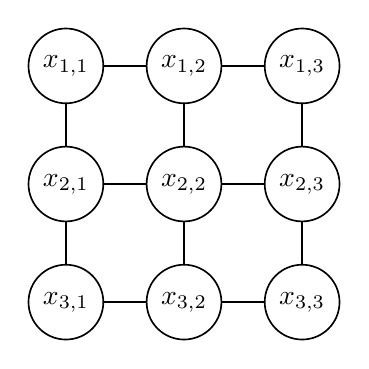
\begin{tikzpicture}[-,minimum size=0.75cm,node distance=1.5cm,semithick]
\tikzstyle{state}=[circle,radius=1cm,fill=white,draw=black,text=black,distance=1cm]
\node[state] (x11)  [] {$x_{1,1}$};
\node[state] (x12) [right  of=x11]{$x_{1,2}$};
\node[state] (x13) [right  of=x12]{$x_{1,3}$};
\node[state] (x21)  [below of=x11] {$x_{2,1}$};
\node[state] (x22) [right  of=x21]{$x_{2,2}$};
\node[state] (x23) [right  of=x22]{$x_{2,3}$};
\node[state] (x31)  [below of=x21] {$x_{3,1}$};
\node[state] (x32) [right  of=x31]{$x_{3,2}$};
\node[state] (x33) [right  of=x32]{$x_{3,3}$};
\path (x11) edge (x12);
\path (x12) edge (x13);
\path (x21) edge (x22);
\path (x22) edge (x23);
\path (x31) edge (x32);
\path (x32) edge (x33);
\path (x11) edge (x21);
\path (x12) edge (x22);
\path (x13) edge (x23);
\path (x21) edge (x31);
\path (x22) edge (x32);
\path (x23) edge (x33);
\end{tikzpicture}
\end{center}
We will index nodes by their row and column, $(2,3)$ is the node in the second row and third column.
When enumerating edges you can iterate each row and column, and consider edges $(i,j) - (i-1,j)$ and
$(i,j) - (i,j-1)$. Hence energy function will look like
\[
E(\xx) = \sum_{(i,j)} \theta(x_{i,j},x_{i-1,j}) + \theta(x_{i,j},x_{i,j-1}) + \psi_{i,j}(x_{i,j}).
\]

Here is a piece of code that can help you compute energy of a configuration in a pairwise MRF
\begin{verbatim}
function E = energy(theta,psi,T,x)
E = 0;
height = size(x,1);
width = size(x,2);
for i=1:height
    for j=1:width
        % unary energy terms are specific to (i,j)
        E = E + psi(x(i,j),i,j);
        if i>1
           E = E + theta(x(i,j),x(i-1,j));
        end
        if j>1
           E = E + theta(x(i,j),x(i,j-1));
        end
    end
end
\end{verbatim}

\paragraph{Grid MRF with observations}
\begin{center}
  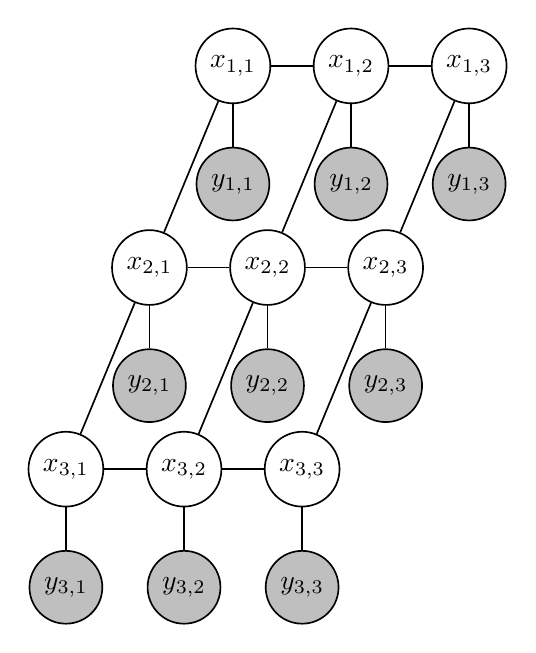
\begin{tikzpicture}[-,minimum size=0.75cm,node distance=1.5cm,semithick]
\tikzstyle{state}=[circle,radius=1cm,fill=white,draw=black,text=black,distance=1cm]
\tikzstyle{observed}=[circle,radius=1cm,fill=lightgray,draw=black,text=black,distance=1cm]
\node[state] (x11)  [] {$x_{1,1}$};
\node[state] (x12) [right  of=x11]{$x_{1,2}$};
\node[state] (x13) [right  of=x12]{$x_{1,3}$};
\node[observed] (y11)  [below of=x11] {$y_{1,1}$};
\node[observed] (y12) [below  of=x12]{$y_{1,2}$};
\node[observed] (y13) [below  of=x13]{$y_{1,3}$};
\node[state] (x21)  [below left of=y11] {$x_{2,1}$};
\node[state] (x22) [right  of=x21]{$x_{2,2}$};
\node[state] (x23) [right  of=x22]{$x_{2,3}$};
\node[observed] (y21)  [below of=x21] {$y_{2,1}$};
\node[observed] (y22) [below  of=x22]{$y_{2,2}$};
\node[observed] (y23) [below  of=x23]{$y_{2,3}$};
\node[state] (x31)  [below left of=y21] {$x_{3,1}$};
\node[state] (x32) [right  of=x31]{$x_{3,2}$};
\node[state] (x33) [right  of=x32]{$x_{3,3}$};
\node[observed] (y31)  [below of=x31] {$y_{3,1}$};
\node[observed] (y32) [below  of=x32]{$y_{3,2}$};
\node[observed] (y33) [below  of=x33]{$y_{3,3}$};
\path (x11) edge (x12);
\path (x12) edge (x13);

\path (x11) edge (y11);
\path (x12) edge (y12);
\path (x13) edge (y13);

\path (x21) edge (x11);
\path (x22) edge (x12);
\path (x23) edge (x13);

\path (x21) edge (x22);
\path (x22) edge (x23);

\path (x21) edge (y21);
\path (x22) edge (y22);
\path (x23) edge (y23);


\path (x31) edge (x21);
\path (x32) edge (x22);
\path (x33) edge (x23);

\path (x31) edge (x32);
\path (x32) edge (x33);

\path (x31) edge (y31);
\path (x32) edge (y32);
\path (x33) edge (y33);

\end{tikzpicture}
\end{center}

We will add observations attached to each node $x_{i,j}$. These are named $y_{i,j}$.
Above graph has a $y$ of size $3 \times 3$.

\paragraph{Joint probability of $\xx,\yy$}
We have specified only probability of $\xx$, but we will now show that we can easily
incorporate the probability of $\yy$ into that formulation.
\[
p(\xx) \propto \myexp{-\frac{1}{T}\sum_{i,j} \theta(x_{i,j},x_{i-1,j}) + \theta(x_{i,j},x_{i,j-1}) + \psi_{i,j}(x_{i,j})}
\]
and
\[
p(\yy|\xx) = \prod_i p(y_{i,j} | x_{i,j})
\]
Joint probability is then
\BEAS
p(\yy,\xx) &\propto& \myexp{-\frac{1}{T}\left(\sum_{i,j} \theta(x_{i,j},x_{i-1,j}) + \theta(x_{i,j},x_{i,j-1}) + \sum_{i,j} \psi_{i,j}(x_{i,j}) - \log p(y_{i,j}|x_{i,j})\right)} \\
           &=& \myexp{-\frac{1}{T}\left(\sum_{i,j} \theta(x_{i,j},x_{i-1,j}) + \theta(x_{i,j},x_{i,j-1}) + \sum_{i,j} \xi_{i,j}(x_{i,j})\right)} \\
\EEAS
where
\[
\xi_{i,j}(x_{i,j)} = \psi_{i,j}(x_{i,j}) - \log p(y_{i,j}|x_{i,j}).
\]
So, even though we changed the name of the unary energy from $\psi$ to $\xi$ there is no real change in the energy computation.
Hence, we can absorb the conditional probabilities $\log p(y_{i,j}|x_{i,j})$ into $\psi$.
Thus energy that corresponds to edge between $x_{i,j}$ and $y_{i,j}$ is incorporated in unary energy $\psi$.
Note the sign flip due to the fact that negative energy is exponentiated in Boltzmann distribution.

\paragraph{Denoising setup} One simple application of pairwise MRFs is in denoising images.
We can think of $\yy$ as a noisy image and $\xx$ a clean version of it.
By sampling
\[
p(\xx|\yy) \propto p(\xx,\yy)
\]
we can obtain configurations from the distribution that puts substantial probability on
the clean, and nearly clean versions of the image.
\begin{figure}
\begin{center}
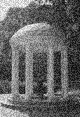
\includegraphics{noisy.png}
\caption{A very noisy image of the old well.}
\end{center}
\end{figure}
\newproblem{2pt}
\paragraph{Specifying $\theta$ and $\psi$}
We will specify a particular $\theta$ and $\psi$
\[
\theta(a,b) = (a - b)^2
\]
and
\[
\psi(a,i,j) = (a - y_{i,j})^2.
\]
Look at the grid MRF above and for $x_{2,2}$ write out all energy terms that involve it:
\answer
There should be 5 of them, since there it has five neighbors.

Interpret what those terms are trying to achieve. You can think about what states
 of $x_{2,2}$ leads to the smallest energy for different states of its neighbors
 \answer

You can use the notion that $x_{2,2}$ is a clean image pixel and $y_{2,2}$ is noisy image
 pixel to explain what is going on.

\newproblem{2pt}
Gibbs sampling iterates updates of single variable at a time, by drawing new
states from conditional probability
\[
p(\xx_{i} | \xx_{[-i]}).
\]
In our case, we need to compute conditional probability
\[
p(x_{i,j} | \xx_{[-(i,j)]},\yy)
\]
First write out the joint probability of $\xx,\yy$ in terms of $\theta$ and $\xi$. Note that $\xi$ is
assumed to have absorbed terms that involve $\yy$.
\[
p(\xx,\yy) = \frac{1}{Z}\myexp{-\frac{1}{T}\left( ... \right)}
\]
Next, identify the terms that depend on $x_{i,j}$ and collect them here
\[
g(x_{i,j},...) = ...
\]
Previous problem should give you guidance on this.

Let the terms that do not involve $x_{i,j}$ be collected in some function $f(\xx_{[-(i,j)]})$ -- you do not need to write it out -- then
we can say that
\[
E(\xx) = g(x_{i,j},...) + f(\xx_{[-(i,j)]}).
\]
Use Bayes rule to obtain
\[
p(x_{i,j}| \xx_{[-(i,j)]},\yy) = \frac{\frac{1}{Z}...}{\frac{1}{Z}...}
\]
Simplify by canceling multiplicative terms that occur in both numerator and denominator.
\[
...
\]
If this looks complicated, for example it involves variables that are not neighbors of $x_{i,j}$, you did something wrong.

\newproblem{2pt}
Take logarithm of the conditional probability and implement code that computes this probability distribution.
You will use logsum
\begin{verbatim}
function p = conditional(x,i,j,theta,xi,T,k)
% x is the current configuration
% i,j are coordinates of variable to update
% theta and xi are energy functions
% T is temperature
% k is the size of state space for each x(i,j)
width = size(x,2);
height = size(x,1);
g = zeros(k,1);

if i>...
   g = g + theta((1:k)',...);
end
if i<...
    g = g + theta((1:k)',...);
end
if j>...
    g = g + theta((1:k)',...);
end
if j<...
    g = g + theta((1:k)',...);
end
g = g + xi((1:k)',i,j);
logp = -1/T*g;
logp = logp - logsum(logp);
p = exp(logp);
\end{verbatim}
To test this out, use
\begin{verbatim}
k = 5;
T = 10;
y = 3*ones(3,3);
xi = @(v,i,j) (v - y(i,j)).^2;
theta = @(a,b) (a-b).^2;
p = conditional(y,2,2,theta,xi,T,k)
\end{verbatim}
You should see something like this
\begin{verbatim}
p =
    0.0545
    0.2442
    0.4026
    0.2442
    0.0545
\end{verbatim}
Implement code that samples from the conditional
\begin{verbatim}
function new = sample(x,i,j,theta,xi,T,k)
p = conditional(x,i,j,theta,xi,T,k)
new = ...
\end{verbatim}

\newproblem{2pt}
A single iteration of Gibbs sampler sweeps through each variable in the model and updates it.
\begin{verbatim}
function gibbs(theta,xi,T,k,y)
% initialize x with noisy image
x = y;
% experiment with different iteration number
for it=1:...
    for i=1:size(x,1)
        for j=1:size(y,1)
            x(i,j) = ...
        end
    end
    figure(1);
    subplot(2,1,1);
    imagesc(x)
    energies(it) = energy(x);
    subplot(2,1,2)
    plot(energies(5:it));
    drawnow
end
\end{verbatim}
Load image in \verb|hw3.mat| and try
\begin{verbatim}
k = max(max(y));
T = 5;
xi = @(v,i,j) (v - y(i,j)).^2;
theta = @(a,b) (a-b).^2;
gibbs(theta,xi,T,k,y)
\end{verbatim}
Experiment with Gibbs sampler using the above update.
You can change temperature, and you can also rescale $\theta$ and $\xi$. 
\begin{verbatim}
xi = @(v,i,j) 2*(v - y(i,j)).^2;
theta = @(a,b) 1/4*(a-b).^2;
\end{verbatim}
Change number of iterations, temperatures, scales of $\theta$ and $\xi$, order of updates. Insert images for different choices of these parameters.
\begin{figure}
\begin{tabular}{ccc}
T=..,iter=..,order=.. & T=..,iter=..,order=.. & T=..,iter=..,order=..\\
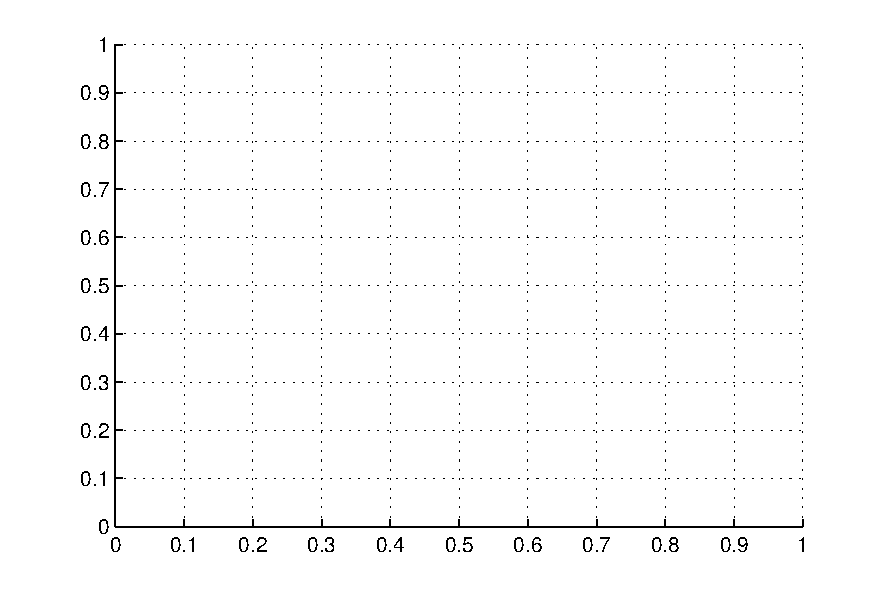
\includegraphics[scale=0.25]{emptiness.pdf}
&

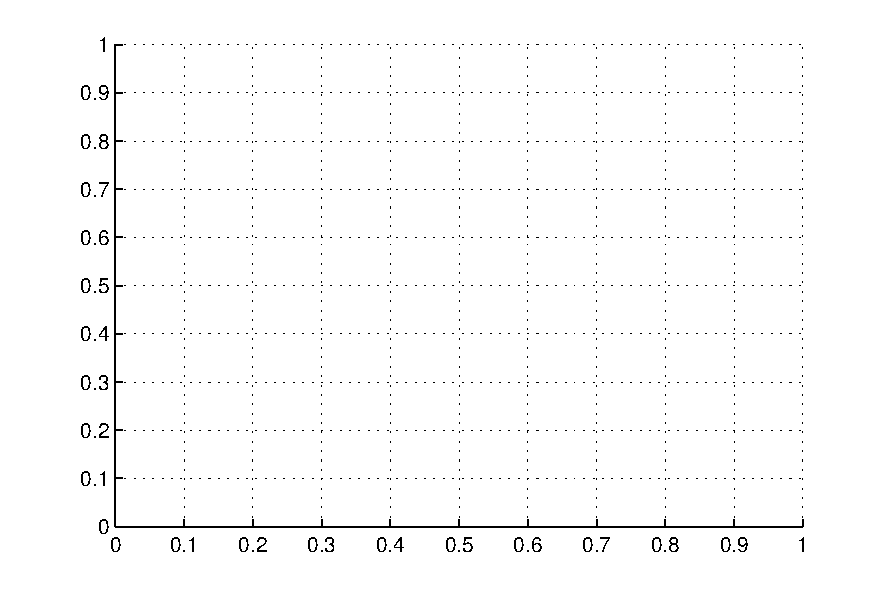
\includegraphics[scale=0.25]{emptiness.pdf}

&

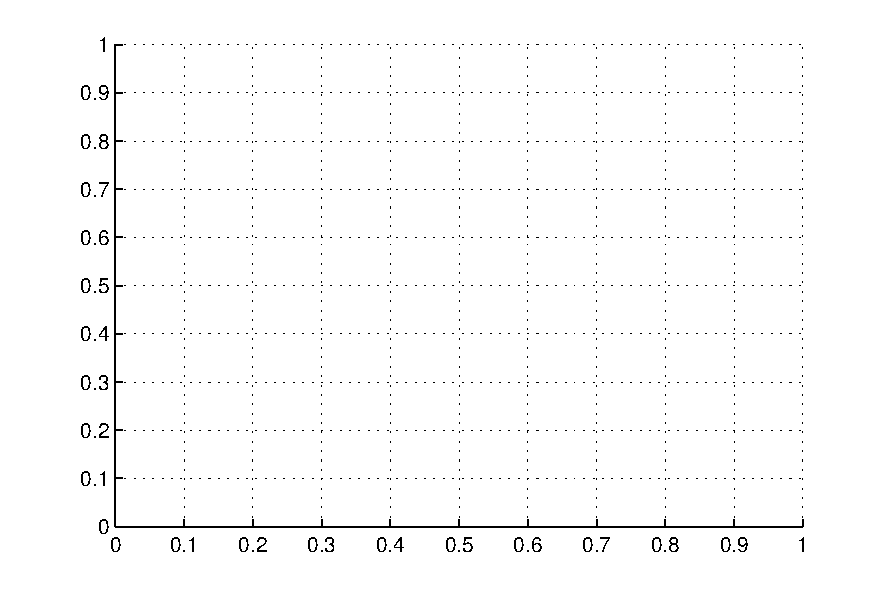
\includegraphics[scale=0.25]{emptiness.pdf}
\end{tabular}
\caption{Denoised images for different settings of parameters ...}
\end{figure}

\newproblem{2pt}
We will now look at the behavior of the chain.
It is common to throw away first iterations of of Gibbs sampler. This is called burn-in

Modify the code to store:
\begin{itemize}
\item the best configuration of $\xx$.
\item store mean of the configurations across all iterations -- you do not need to store all the
configurations to compute the mean.
\item store mean of the configurations across all iterations after iteration B
\item compute per pixel variance in configurations
\end{itemize}

Show the best image, mean image across all iterations, mean after burn-in, variance
after burn-in.
\begin{figure}
\begin{tabular}{ccc}
Best & Mean & Mean after burnin\\
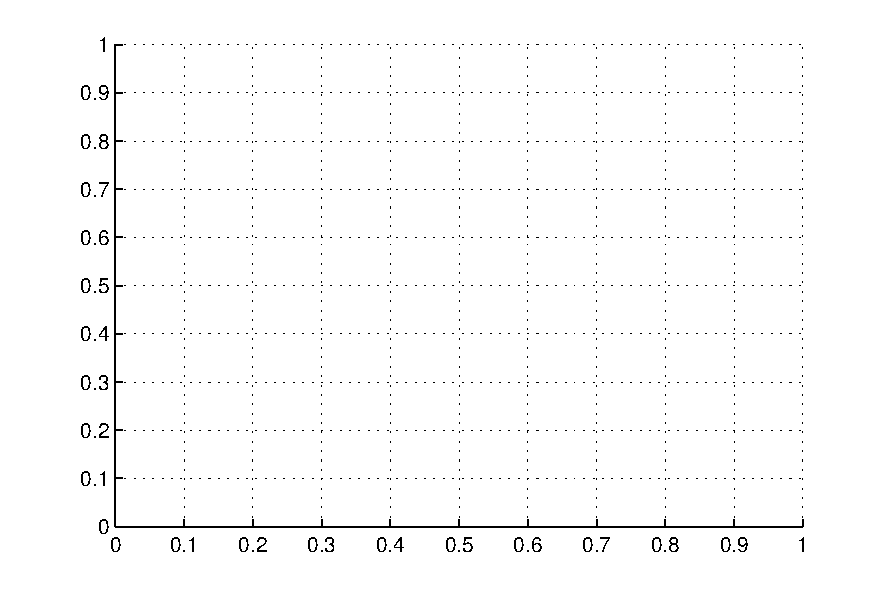
\includegraphics[scale=0.25]{emptiness.pdf}
&

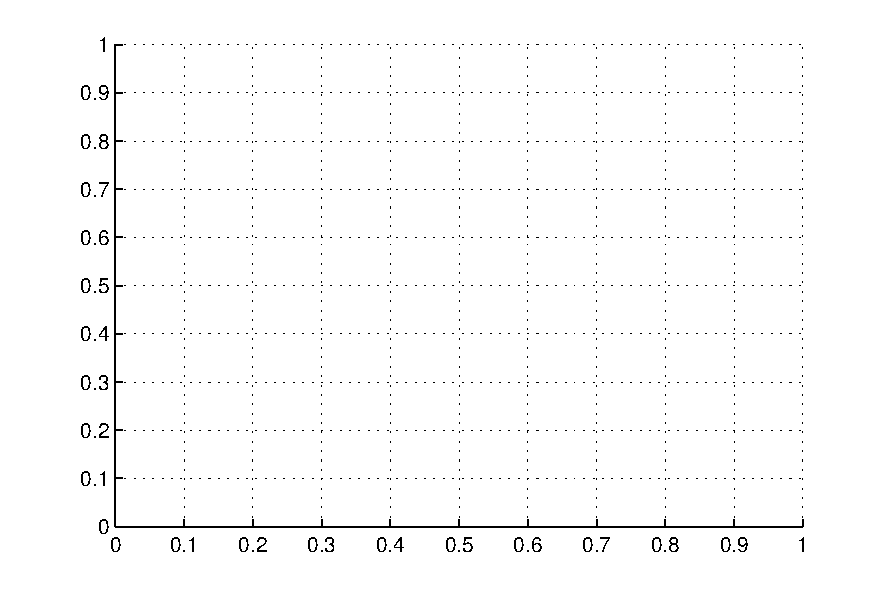
\includegraphics[scale=0.25]{emptiness.pdf}

&

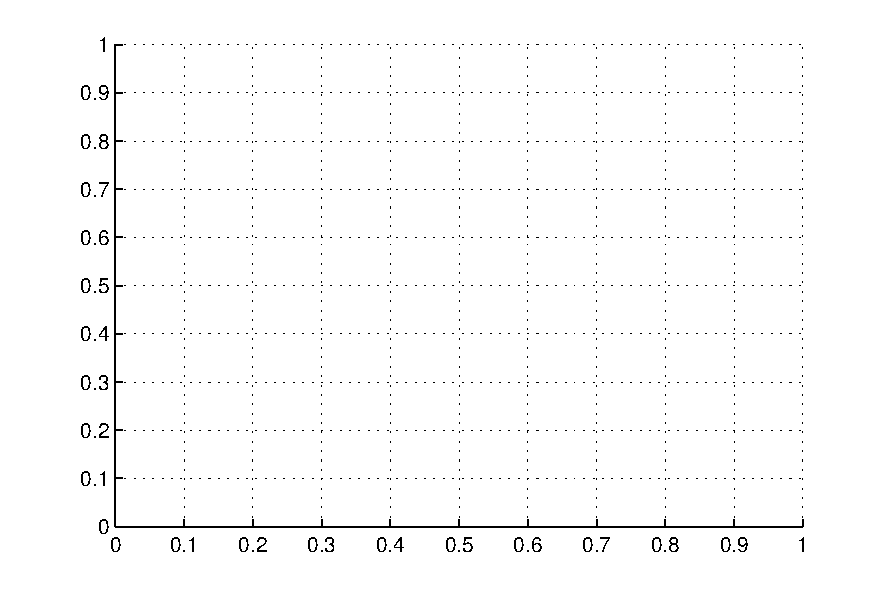
\includegraphics[scale=0.25]{emptiness.pdf}
\end{tabular}
\end{figure}

\newproblem{2pt} Choose the temperature, number of iterations and burn-in that seems to perform well.
Change initialization of $\xx$ to be random.
Start 5 chains -- all from different initial configurations--, collect the energies plots across all the iterations and plot them in the same plot but
using different colors.
Do all chains reach roughly the same energy levels? If not, run them for a longer time.
Once you have the chains behaving similarly -- they are mixing -- generate the plot and add it below.
\begin{figure}
\begin{center}
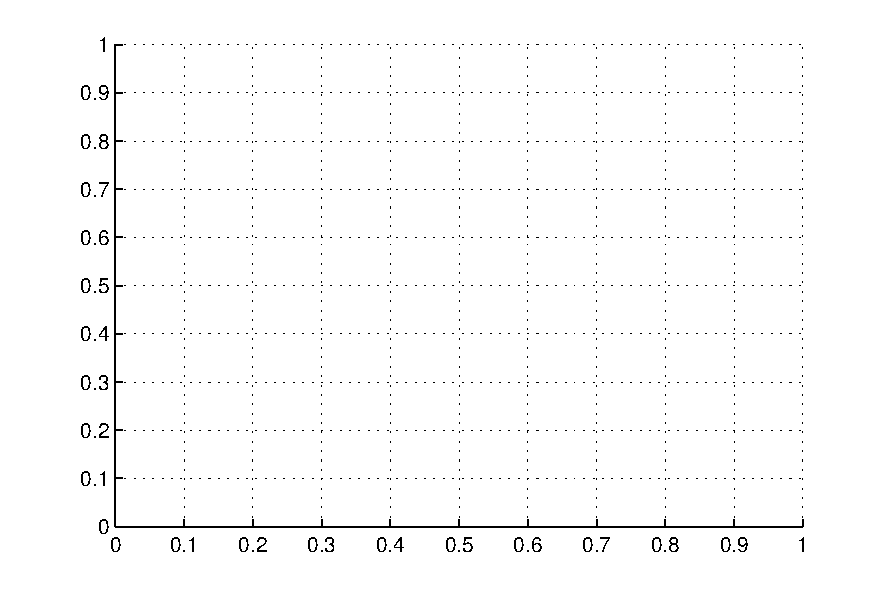
\includegraphics{emptiness.pdf}
\caption{Energies across Gibbs iterations of 5 chains}
\end{center}
\end{figure}


\begin{figure}
\begin{center}
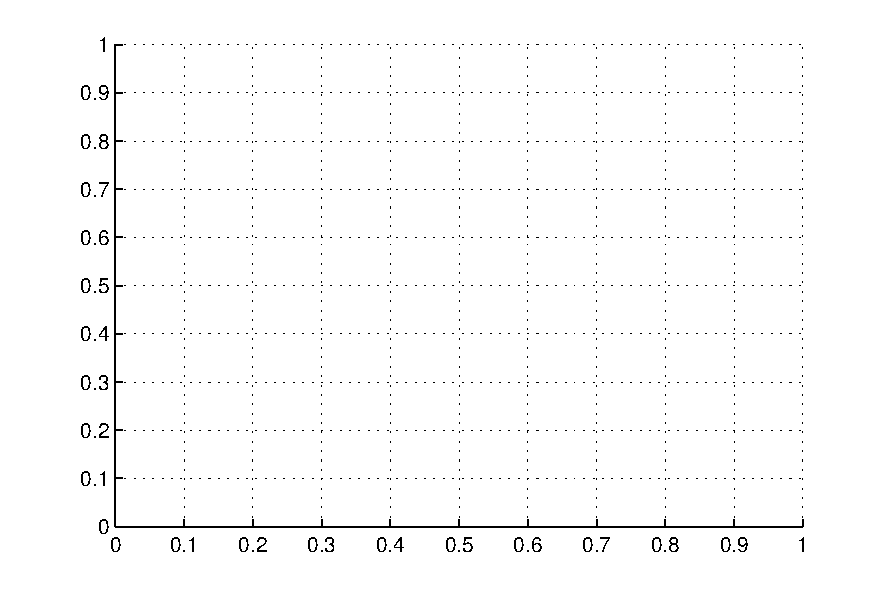
\includegraphics{emptiness.pdf}
\end{center}
\caption{Denoised image}
\end{figure}



\end{document}
